% 1_introduction.tex

\cleardoublepage
\chapter{Introduction}


  	\begin{figure}
  		\centering
  		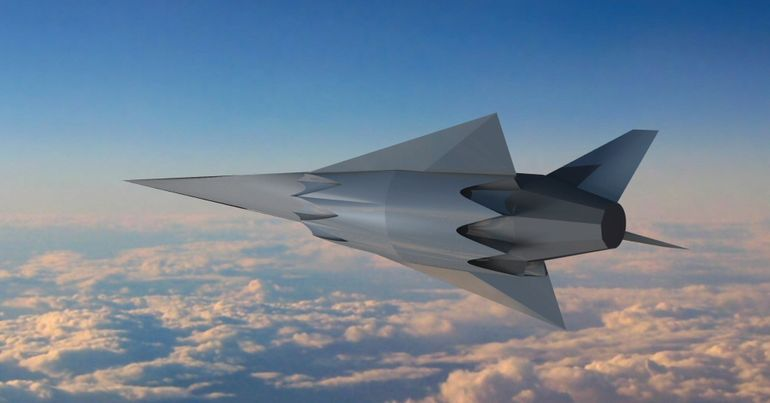
\includegraphics[width=0.7\linewidth]{figures/1_introduction/project-spartan}
  		\caption{}
  		\label{fig:project-spartan}
  	\end{figure}
  	
  	  Airbreathing engines are an ideal candidate for producing the next generation of space access
  	systems. Airbreathing engines produce higher specific impulse than rockets, and require far less propellant to be carried on-board a launch vehicle. 
  	 The mass savings gained by using airbreathing engines allow launch vehicles to be designed to be reusable, capable of manoeuvring aerodynamically and of landing similarly to a conventional aircraft. A three stage design utilising a scramjet
  	second stage with rocket powered first and third stages is being developed by The University of
  	Queensland. In previous studies it has been assumed that the optimal trajectory for a scramjet powered vehicle is at its
  	maximum dynamic pressure and all other trajectory stages have conformed to this assumption. This study will aim to produce an optimal
  	trajectory plan which may be applied to any rocket-airbreathing-rocket system for delivering small
  	satellites to Earth orbit. The SPARTAN vehicle being developed by the university of Queensland will
  	be used as a model for simulations.
  	\textcolor{red}{focus on my achievements, rather than justifying small satellite launchers}
  	
  
  
  The SPARTAN is being developed to take advantage of a rapidly increasing market for small satellite launches.
  Many small satellites are currently launched with multiple small satellites piggybacking onto the launch of larger satellites, comanifesting on a single launch to share costs. This has the result
  of smaller payloads being subject to the schedule of the other parties involved, and being delivered into
  an orbit determined by the requirements of the main payload. This dependence on a predetermined mission plan often has detrimental effects on the small satellite mission. Small satellites are often used in missions which require specific orbital and scheduling needs. Satellites to be used as part of constellations are especially sensitive to the orbit in which they are placed. Small satellites may be able to change orbits slightly, however larger changes mean additional fuel mass and potentially additional system mass if a larger drive is necessary. 
  The production of a cheap and flexible small satellite delivery system would enable more small satellites to be delivered into customised orbits within relatively short time periods.
  \textcolor{red}{rephrase, comment on limited fuel availability}
  

  	\textcolor{red}{Add image of the final trajectory}
  \section{Research aims}

    The overall aim of this thesis is to apply state of the art numerical optimisation techniques to the trajectory of a rocket-scramjet-rocket small satellite launch system. The purpose of this optimised trajectory is to maximise the payload-to-orbit capabilities of the launch system, thereby also maximising the cost efficiency of the system. 
    
    \textcolor{red}{add more, flexibility, turn around time, operability}
    

    \noindent This will be achieved through the following objectives:
 \textcolor{red}{IJ - not objectives, redo}
    \begin{enumerate}
    	 \item \emph{Third stage redesign.}\\
    	 To ensure that the simulated system is representative of an up-to-date, relevant design,
    	 the third stage of the rocket-scramjet-rocket launch system is to be redesigned to use the Kestrel pressure-fed engine. This redesign requires the third stage  shape and internal layout to be changed considerably, as well as the second stage internal layout to be reconfigured. 

\item \emph{First stage design.}\\
		The first stage has not yet been studied previously, and as such a representative design of a first stage rocket is created. 
    	
      \item \emph{Launch system simulation.}\\
      A thorough numerical simulation of the launch system is created, which fits into the format required by the optimisation algorithm. 

      \item \emph{Optimisation integration}\\



    \end{enumerate}

  \clearpage
  \section{Thesis outline}

    Edit this as required. This thesis is organised in eight chapters which are outlined below. The appendices included at the end of this document contain further technical information and supplementary experimental details. \textcolor{red}{If you want to add colours to the text for some reason (supervisor reviewing etc.), use the \texttt{textcolor} command. Check the code here to see how.}

    \subsubsection*{Chapter 2 -}

      This chapter presents a review of literature related to the different aspects of this thesis. 

    \subsubsection*{Chapter 3 - }

      This chapter provides details of the 

    \subsubsection*{Conclusions}

      The body of this thesis concludes by summarising the most significant findings from
